%% Los cap'itulos inician con \chapter{T'itulo}, estos aparecen numerados y
%% se incluyen en el 'indice general.
%%
%% Recuerda que aqu'i ya puedes escribir acentos como: 'a, 'e, 'i, etc.
%% La letra n con tilde es: 'n.

\chapter{Marco contextual}
\section*{Introducci'on}
\addcontentsline{toc}{section}{Introducci'on}

En 'este cap'itulo se describen algunos marcos conceptuales necesarios para fundamentar y analizar los requisitos de la investigaci'on, las secciones son las siguientes: Situaci'on actual, Estado del Arte, Marco Te'orico y Marco Metodol'ogico. En la primera secci'on se muestra c'omo se encuentra la investigaci'on en la actualidad, c'omo se encuentra nacional e internacionalmente y cu'al es el punto de partida del proyecto; en la siguiente secci'on se presenta la informaci'on sobre los diferentes esquemas de distribuci'on que ser'an implementados durante la elaborac'on del proyecto. El Marco te'orico nos describe los conceptos necesarios para fundamentar y comprender mejor el proyecto y su prop'osito, finalmente en la 'ultima secci'on se describe los pasos que se van a seguir para realizar y alcanzar los objetivos del proyecto.

\newpage


\section{Situaci'on Actual}

Actualmente, son muchas las organizaciones que utilizan el c'omputo en la nube, ya que trae beneficios en cuanto a gastos y recursos. Ya no hay necesidad de invertir tanto en la infraestructura de \textit{TI (Information Technology)} y existe una mejor capacidad de almacenamiento para los recursos que el 'ambito empresarial necesita.
El c'omputo en la nube utiliza los servicios \textit{SaaS (Software as a Service)} y \textit{HaaS (Hardware as a Service)} para hacer m'as eficiente y flexible el uso de la infraestructura de la nube (\citeauthor{mariscal2013computo}, \citeyear{mariscal2013computo}). 

M'exico utiliza, en cuanto a la infraestructura de almacenamiento virtual, los servicios ofrecidos por \textit{Amazon, Google y Triada (TELMEX)}. Los cuales proporcionan almacenaje de informaci'on virtual, plataformas de hospedaje de aplicaciones y servicios en l'inea (\citeauthor{mariscal2013computo}, \citeyear{mariscal2013computo}).

Al proveer el servicio se tiene dos escenarios diferentes: cuando hay una mayor demanda de recursos y cuando no la hay,  eso va dependiendo de las necesidades de las empresas. 
Para que se tenga una mejor eficacia durante los servicios, se tiene que mejorar el uso de los recursos en el centro de datos. Dentro del centro de datos hay muchos servidores virtuales que est'an recibiendo trabajos, mientras la nube las mantiene en los lotes de solicitud de trabajos. Es aqu'i, donde resaltamos la importancia de la distribuci'on de trabajos dentro del centro de datos (\citeauthor{shimpy2014different}, \citeyear{shimpy2014different}). 

En este momento, la distribuci'on de trabajos es un problema NP- dif'icil, pues que no se ha encontrado una soluci'on 'optima. Sin embargo, existen diferentes propuestas para encontrar una mejor soluci'on, utilizando diferentes esquemas de distribuci'on o dicho de otra forma algoritmos (\citeauthor{shimpy2014different}, \citeyear{shimpy2014different}). 

Existen una gran variedad de algoritmos utilizados en el problema de distribuci'on de trabajos. Los algoritmos m'as utilizados en las investigaciones son: \textit{FCFS, Round Robin, Min-Min, Max-Min y Metaheur'istica}. Cabe mencionar que en las investigaciones solo hacen una selecci'on de una serie de algoritmos para que, por medio de pruebas, determinen qui'en es el mejor de ellos. 


\newpage
\section{Estado del Arte}


Los siguientes algoritmos de calendarizaci'on actualmente est'an prevaleciendo en la nube:
\begin{itemize}
	\item \textit{\textbf{Resource-Aware-Scheduling Algorithm (RASA):}} Parsa, Entezari-Maleki (2009) proponen el algoritmo \textit{RASA}, el cual utiliza las ventajas de dos algoritmos tradicionales \textit{(Max-min y Min-min)} y cubre sus desventajas. Aunque el tiempo limite, la tasa de llegada, costo de ejecución y costo de comunicaci'on no est'an considerados (\citeauthor{parsa2009rasa}, \citeyear{parsa2009rasa}).
	
	
	\item \textit{\textbf{RSDC (Reliable Scheduling Distributed In Cloud Computing):}} Delevar, Javanmard, Shabestari y Talebi (2012) proponen un algoritmo confiable en un entorno en la nube, en este algoritmo los trabajos importantes son divididos en sub trabajos, de tal manera que se puedan balancear las peticiones (\citeauthor{delavar2012rsdc}, \citeyear{delavar2012rsdc}).
	
	
	\item \textit{\textbf{An Optimal Model for Priority based Service Scheduling Policy for Cloud Computing Environment:}} Dakshayini, Gurupased (2011), proponen un nuevo algoritmo de calendarizaci'on que se basa en la prioridad y un esquema de control de admisi'on. En este algoritmo, la prioridad se asigna a cada proceso admitido en la cola (\citeauthor{dakshayini2011optimal}, \citeyear{dakshayini2011optimal}) . 
	
	
	\item \textit{\textbf{Pre-emptable Shortest Job Next Scheduling algorithm (PSJN) :}}  Este algoritmo se propone en una nube privada. Utiliza la t'ecnica de suscripci'on preferente del algoritmo de \textit{Round Robin} junto con el siguiente proceso m'as corto \textit{(PSN)}. Brinda beneficios de costos y mejora tiempo de respuesta y tiempo de ejecuci'on (\citeauthor{nishant}, \citeyear{nishant}). 
	
	
	\item \textit{\textbf{User-priority Guided Min-min scheduling algorithm:}} Se realiza una mejora para el algoritmo de balanceo de cargas, a trav'es del algoritmo \textit{Min-min} para la calendarizaci'on de trabajos con el fin de minimizar el tiempo de terminaci'on del ultimo trabajo \textit{(makespan)} y maximizar la utilizaci'on de los recursos (\citeauthor{chen2013user}, \citeyear{chen2013user}). 
\end{itemize}



\section{Marco te'orico}

El c'omputo en la nube es una tecnolog'ia emergente, la cual est'a compuesta por un grupo de recursos heterog'eneos que proveen servicios a trav'es de internet (\citeauthor{agarwal2014efficient}, \citeyear{agarwal2014efficient}).
Esta tecnolog'ia permite a los consumidores y negocios utilizar aplicaciones sin necesidad de instalaci'on y con acceso a sus archivos personales en cualquier computadora con acceso a internet (\citeauthor{ahmed2012advanced}, \citeyear{ahmed2012advanced}). 
El c'omputo en la nube se puede clasificar de dos maneras:
\begin{itemize}
	\item Por la ubicaci'on: 
	\begin{itemize}
		\item \textbf{Nube P'ublica:} La infraestructura de c'omputo se puede compartir entre cualquier organizaci'on (\citeauthor{ahmed2012advanced}, \citeyear{ahmed2012advanced}).
		\item \textbf{Nube Privada:} La infraestructura de c'omputo es dedicada a una organizaci'on en particular y no se comparte con otras organizaciones (\citeauthor{ahmed2012advanced}, \citeyear{ahmed2012advanced}).
		\item \textbf{Nube H'ibrida:} Las organizaciones pueden albergar sus aplicaciones cr'iticas en nubes privadas y las aplicaciones con menos problemas de seguridad las puede albergar en nubes p'ublicas (\citeauthor{ahmed2012advanced}, \citeyear{ahmed2012advanced}).
	\end{itemize}
	\item Por el tipo de servicios ofrecidos: 
	\begin{itemize}
		\item \textit{\textbf{Infrastructure as a Service (IaaS):}} En 'este nivel, la infraestructura se ofrece como servicio hacia los solicitantes en forma de M'aquinas Virtuales \textit{(VM)} (\citeauthor{agarwal2014efficient}, \citeyear{agarwal2014efficient}).
		\item \textit{\textbf{Platform as a Service (PaaS):}} Es una plataforma de desarrollo de aplicaciones que se provee como servicio hacia los desarrolladores para crear aplicaciones basadas en web (\citeauthor{agarwal2014efficient}, \citeyear{agarwal2014efficient}).
		\item \textit{\textbf{Software as a Service (SaaS):}} En 'este nivel el proveedor en la nube provee las aplicaciones de \textit{software} (\citeauthor{agarwal2014efficient}, \citeyear{agarwal2014efficient}).
	\end{itemize}
\end{itemize}




\setcounter{figure}{1}
\renewcommand\thefigure{\arabic{figure}}
\begin{figure}
	\centering
	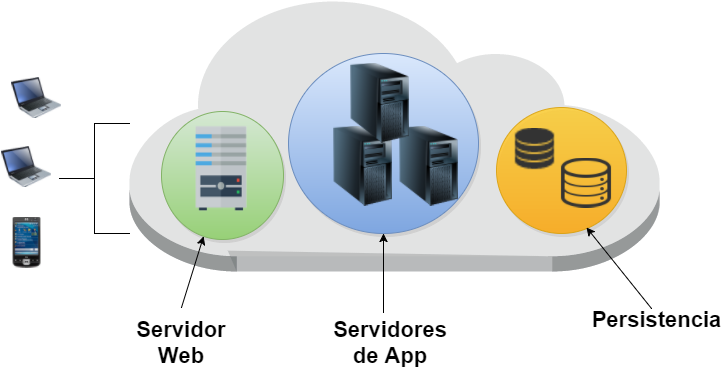
\includegraphics[scale=0.5]{media/cloud1}
	\caption{Esquema general del C'omputo en la Nube, Fuente: Elaboraci'on propia.}
\end{figure}


\subsection*{Centro de Datos}
\addcontentsline{toc}{subsection}{Centro de Datos}
Un centro de datos \textit{(datacenter)} es un espacio dedicado donde las organizaciones almacenan y operan la mayor'ia de su informaci'on y la infraestructura de las tecnolog'ias de comunicaciones que respaldan sus negocios (\citeauthor{whatisdatacenter}, \citeyear{whatisdatacenter}).

\subsection*{Esquemas de Distribuci'on de Trabajos}
\addcontentsline{toc}{subsection}{Esquemas de Distribuci'on de Trabajos}

La distribuci'on de trabajo (calendarizaci'on) es uno de los puntos principales adem'as de los m'as retadores problemas en el c'omputo en la nube (\citeauthor{li2014greedy}, \citeyear{li2014greedy}). Esta consiste en un conjunto de pol'iticas para controlar el orden en el cual los procesos ser'an ejecutados por el sistema (\citeauthor{agarwal2014efficient}, \citeyear{agarwal2014efficient}).

Existen varios tipos de algoritmos de calendarizaci'on, su principal ventaja es obtener un alto rendimiento al cumplir con las trabajos. Los principales ejemplos de algoritmos de calendarizaci'on son (\citeauthor{salot2013survey}, \citeyear{salot2013survey}):

\begin{itemize}
	\item \textit{\textbf{FCFS (First Come First Serve) Algorithm:}} significa que el trabajo que llegue primero ser'a el primero en ser ejecutado.
	\item \textit{\textbf{Round Robin Algorithm:}} consiste en agregar un tiempo de ejecuci'on para cada trabajo, si dicho tiempo se agota y el trabajo actual no ha finalizado, pasa a un estado de espera y contin'ua con el siguiente trabajo, al finalizar el 'ultimo trabajo regresa a revisar si existen trabajos en espera para proceder a ejecutarlas. 
	\item  \textit{\textbf{Min-Min Algorithm:}} se va ejecutando una por una iniciando por los trabajos de menor tama'no.
	\item  \textit{\textbf{Max-Min Algorithm:}} se va ejecutando una por una iniciando por los trabajos de mayor tama'no.
	\item  \textit{\textbf{Most fit task scheduling algorithm:}} este algoritmo busca los elementos m'as aptos en la cola de trabajos para ejecutarlo primero. Tiene un alto radio de error.
	\item \textit{\textbf{Priority scheduling algorithm:}} la idea b'asica es que a cada proceso se le asigna una prioridad, y dependiendo a las prioridades de los dem'as procesos es c'omo se ejecutar'an cada uno de ellos.
\end{itemize}

\subsection*{Balanceo de Cargas}
\addcontentsline{toc}{subsection}{Balanceo de Cargas}

Dentro de nuestro entorno en la nube cada \textit{host} tiene recursos de \textit{hardware} finitos y son susceptibles a fallos. Para mitigar contra las fallas y el exhaustivo uso de los recursos, los \textit{host} son agrupados en \textit{clusters}, los cuales son esencialmente un agrupamiento de recursos compartidos. El administrador \textit{(manager)} es capaz de asegurarse que ninguno de los \textit{host} dentro del \textit{cluster} es responsable de todas las m'aquinas virtuales dentro de ese \textit{cluster} (\citeauthor{redhat}, \citeyear{redhat}).

Un entorno de virtualizaci'on responde a los cambios en la demanda para los recursos en cada host haciendo uso del balanceo de cargas, calendarizaci'on de trabajos y migraci'on.

Una pol'itica de balanceo de cargas es configurada para un \textit{cluster}, que a su vez contiene multiples \textit{hosts}, cada uno de ellos con distintos recursos de \textit{hardware} y disponibilidad de memoria (\citeauthor{redhat}, \citeyear{redhat}). 


Existen tres pol'iticas para el balanceo de cargas:
\begin{itemize}
	\item Sin Balanceo.
	\item Distribuci'on Uniforme.
	\item Ahorro de Energ'ia.
\end{itemize}

\subsection*{Migraci'on}
\addcontentsline{toc}{subsection}{Migraci'on}

La migraci'on se utiliza para hacer cumplir las pol'iticas dentro del balanceo de cargas. La migraci'on de una m'aquina virtual toma lugar de acuerdo a las pol'iticas de balanceo de cargas para un \textit{cluster} y la demanda actual sobre los \textit{hosts} dentro de dicho \textit{cluster}. La migraci'on de igual manera puede ser configurada para ocurrir autom'aticamente cuando un \textit{host} es bloqueado o movido a modo de mantenimiento (\citeauthor{redhat}, \citeyear{redhat}).
\subsection*{Sistemas \textit{ERP}}
\addcontentsline{toc}{subsection}{Sistemas ERP}

La sigla \textit{ERP}, en ingl'es \textit{Enterprise Resource Planning}, significa Planificaci'on de los Recursos de la Empresa. Un sistema \textit{ERP} constituye un marco de trabajo que incluye aplicaciones comerciales, administrativas (finanzas, contabilidad), recursos humanos, planeamiento de manufactura y gesti'on de proyectos (\citeauthor{saroka2002sistemas}, \citeyear{saroka2002sistemas}). 


\section{Marco Metodol'ogico}

A continuaci'on se propone la siguiente metodolog'ia para llevar a cabo el proyecto:

\begin{itemize}
	\item \textbf{Simular:} Se implementar'a a manera de simulaci'on un centro de datos con un entorno en la nube, las m'aquinas virtuales y el servidor inicializador que lo conforman.
	\item \textbf{Implementar:} En el centro de datos se desarrollar'an los algoritmos de calendarizaci'on que se mencionan con antelaci'on.
	\item \textbf{Evaluar:} Se simular'a el comportamiento de las peticiones de un sistema contemplando los distintos escenarios del \textit{ERP} y consumiendo el servicio en la nube \textit{(SaaS)}, para conocer el rendimiento en tiempo de ejecuci'on de los algoritmos.
	\item \textbf{Mejorar:} Se propondr'a una mejora a alg'un algoritmo de acuerdo a las necesidades y comportamiento de un sistema \textit{ERP} en la nube.
	\item \textbf{Comparar:} Se realizar'a una comparativa de tiempo de ejecuci'on entre la versi'on mejorada y la original para el caso de estudio de un sistema \textit{ERP}.
\end{itemize}




